\documentclass{article}
\usepackage[utf8]{inputenc}
\usepackage{amsmath}


\title{SciComp2017 HW2}
\author{Dmitriy Salnikov}
\date{October 2017}

\usepackage{natbib}
\usepackage{graphicx}

\newcommand\norm[1]{\left\lVert#1\right\rVert}

\begin{document}

\maketitle

\section{Problem1}
\subsection{1}
For $A_q$ the condition number can be calculated as $\sqrt{\frac{\lambda_{max}}{\lambda_{min}}}$ where $\lambda$ is the set of eigenvalues of $A_q^{T}*A_q$. After calculating the characterisic polinomial and solving for $\lambda$ we get. 

 \[ 
k(A_q) = 
\frac{\max\left(\frac{\sqrt{2}}{2} \sqrt{q^{2} - q \sqrt{q^{2} + 4} + 2}, \frac{\sqrt{2}}{2} \sqrt{q^{2} + q \sqrt{q^{2} + 4} + 2}\right)}{\min\left(
\frac{\sqrt{2}}{2} \sqrt{q^{2} - q \sqrt{q^{2} + 4} + 2}, \frac{\sqrt{2}}{2} \sqrt{q^{2} + q \sqrt{q^{2} + 4} + 2}\right)}
\]

\subsection{2}

If we take \[ b = (10^7, 1), \Delta{b} = (1, 0), q = 10^7\] then 
\[ x = (0, 1), \Delta{x} = (1, 0)\] and we get 

\[
\frac{\norm{\Delta{x}}}{\norm{x}} = 1 \ge \frac{10^6}{10^{14} + 1} = \frac{\norm{\Delta{b}}}{\norm{b}}
\]


\section{Problem2}
The first formula has the first order  error 

Since,
\[
    f( x + h ) = f(x) + f'(x)h + O(h^2)
\]
then 
\[
    f'(x) \approx \frac{f(x+h) - f(x)}{h} = f'(x) + O(h)
\]

If function is twice differentiable, with the second formula we get
\[
f( x + h ) = f(x) + f'(x)h + \frac{f''(x)h}{2} + O(h^3)
\]

\[
f( x - h ) = f(x) - f'(x)h + \frac{f''(x)h}{2} + O(h^3)
\]

then

\[
    f'(x) \approx \frac{f(x+h) - f(x-h)}{2h} = f'(x) + O(h^2)
\]

Experimental results confirm that and ,until precision errors come into play, we can see a steeper decline of the approximation error.

The minimum for the first approximation is achieved at $h10^{-8}$ and equals $2.554135347665465e-08$. For the centered formula the minimum is achieved at $10^{-7}$ and equals $6.2239102760486276e-12$

\begin{figure}[h!]
\centering
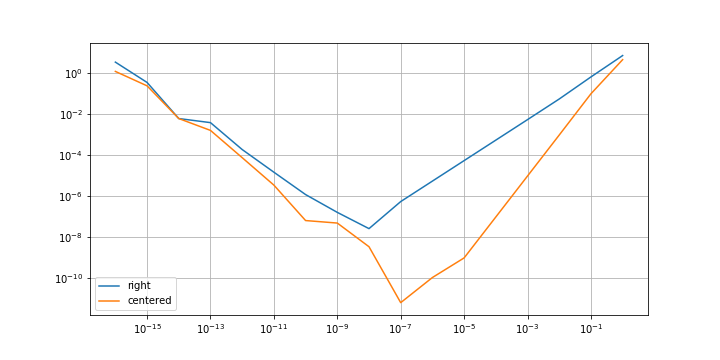
\includegraphics[scale=0.5]{errorplot.png}
\caption{Error graphs}
\label{fig:error_graph}
\end{figure}


\section{Problem3}



\section{Problem4}
By Taylor expansion, the local approximation order is $O(\Delta{t}^3)$

\[
x(t + \Delta{t}) = x(t) + v\Delta{t} + \frac{1}{2}f(t)\Delta{t}^2 + O(\Delta{t}^3) 
\]

Substituting first equation into the second one we get

\[
x(t + \Delta{t}) = x(t) + (v(t) + \frac{1}{2}f(t)\Delta{t})\Delta{t}
\]

\[
x(t+ \Delta{t}) = x(t) + v\Delta{t} + \frac{1}{2}f(t)\Delta{t}^2
\]

So, subtracting this from the Tailor expansion we get the the desired approximation order.
Then, the global approximation order is $\frac{C}{t} * O(\Delta{t}^3) = O(\Delta{t}^2)$
Please find the experiments in the corresponding jupyter notebook



\section{Problem5}
Please see the attached notebook for the implementations and comparison. Algorithm performs grid search in order to find the best regulatization parameter. In terms of error, works similar to $sklearn.linear_model.LinearRegression$ on one dataset, and performs better on the other one.

% \bibliographystyle{plain}
% \bibliography{references}
\end{document}
